% 
% Licensed to the Apache Software Foundation (ASF) under one
% or more contributor license agreements.  See the NOTICE file
% distributed with this work for additional information
% regarding copyright ownership.  The ASF licenses this file
% to you under the Apache License, Version 2.0 (the
% "License"); you may not use this file except in compliance
% with the License.  You may obtain a copy of the License at
% 
%   http://www.apache.org/licenses/LICENSE-2.0
% 
% Unless required by applicable law or agreed to in writing,
% software distributed under the License is distributed on an
% "AS IS" BASIS, WITHOUT WARRANTIES OR CONDITIONS OF ANY
% KIND, either express or implied.  See the License for the
% specific language governing permissions and limitations
% under the License.
% 

% \section{DUCC Service Manager}
    This section describes the architecture and internal structure of the
    DUCC Service Manager, referred to as the ``SM''.

\section{Introduction}
    The SM function is to insure that any services needed by
    DUCC jobs are running and functional at the time they are needed by
    jobs.  Previous to the incarnation of the SM it was necessary for
    users to manually invoke the processes implementing their services.  If
    these processes were to crash, jobs dependent on them would stop until
    some human was able to restart the service.  If the operating system,
    or batch system supporting the jobs (DUCC, in our case) was to
    be restarted, users would again have to manually start the services.

    By ``registering'' a service with the SM, a user can trust DUCC to
    keep the service alive and functional across all manner of faults and
    system restarts.  As well, the SM has a mechanism for ``testing'' a
    service to determine if it is operational, and to inform the DUCC
    Web Server when it is not.  

    If a user submits a job that declares a dependency on a service, the SM
    is able to start the service as needed, and is able to stop the service
    when no longer needed, freeing resources.

    In essence, the SM can be thought of as a ``proxy user'' dedicated
    to insuring that services are always available when needed.

\section{Architectural Overview}

    Figure ~\ref{fig:sm-structure} below shows the high-level object,
    threading, and process structure of SM and should be referenced
    while reading this document.
    
    The SM can be pictured as being composed of four major parts:
    \begin{enumerate}
      \item Initialization and interaction with external components.
        External components include user requests and  other DUCC components such as
        the Orchestrator.
      \item A ``Service Instance'' manager.  This part resolves
        dependencies on services, starts and stops service instances
        according to the needs of jobs and the policies declared in
        the service registries, and handles the service instance
        lifetimes.
      \item A ``Service Health'' manager.  This part continually
        ``tests'' services to determine whether they are 
        functional.  This is referred to as the ``pinger'' and the
        test is known as a ``ping''.
      \item A ``CLI Handler'' which reacts to requests from users.
    \end{enumerate}

    \begin{figure}[H]
      \centering
      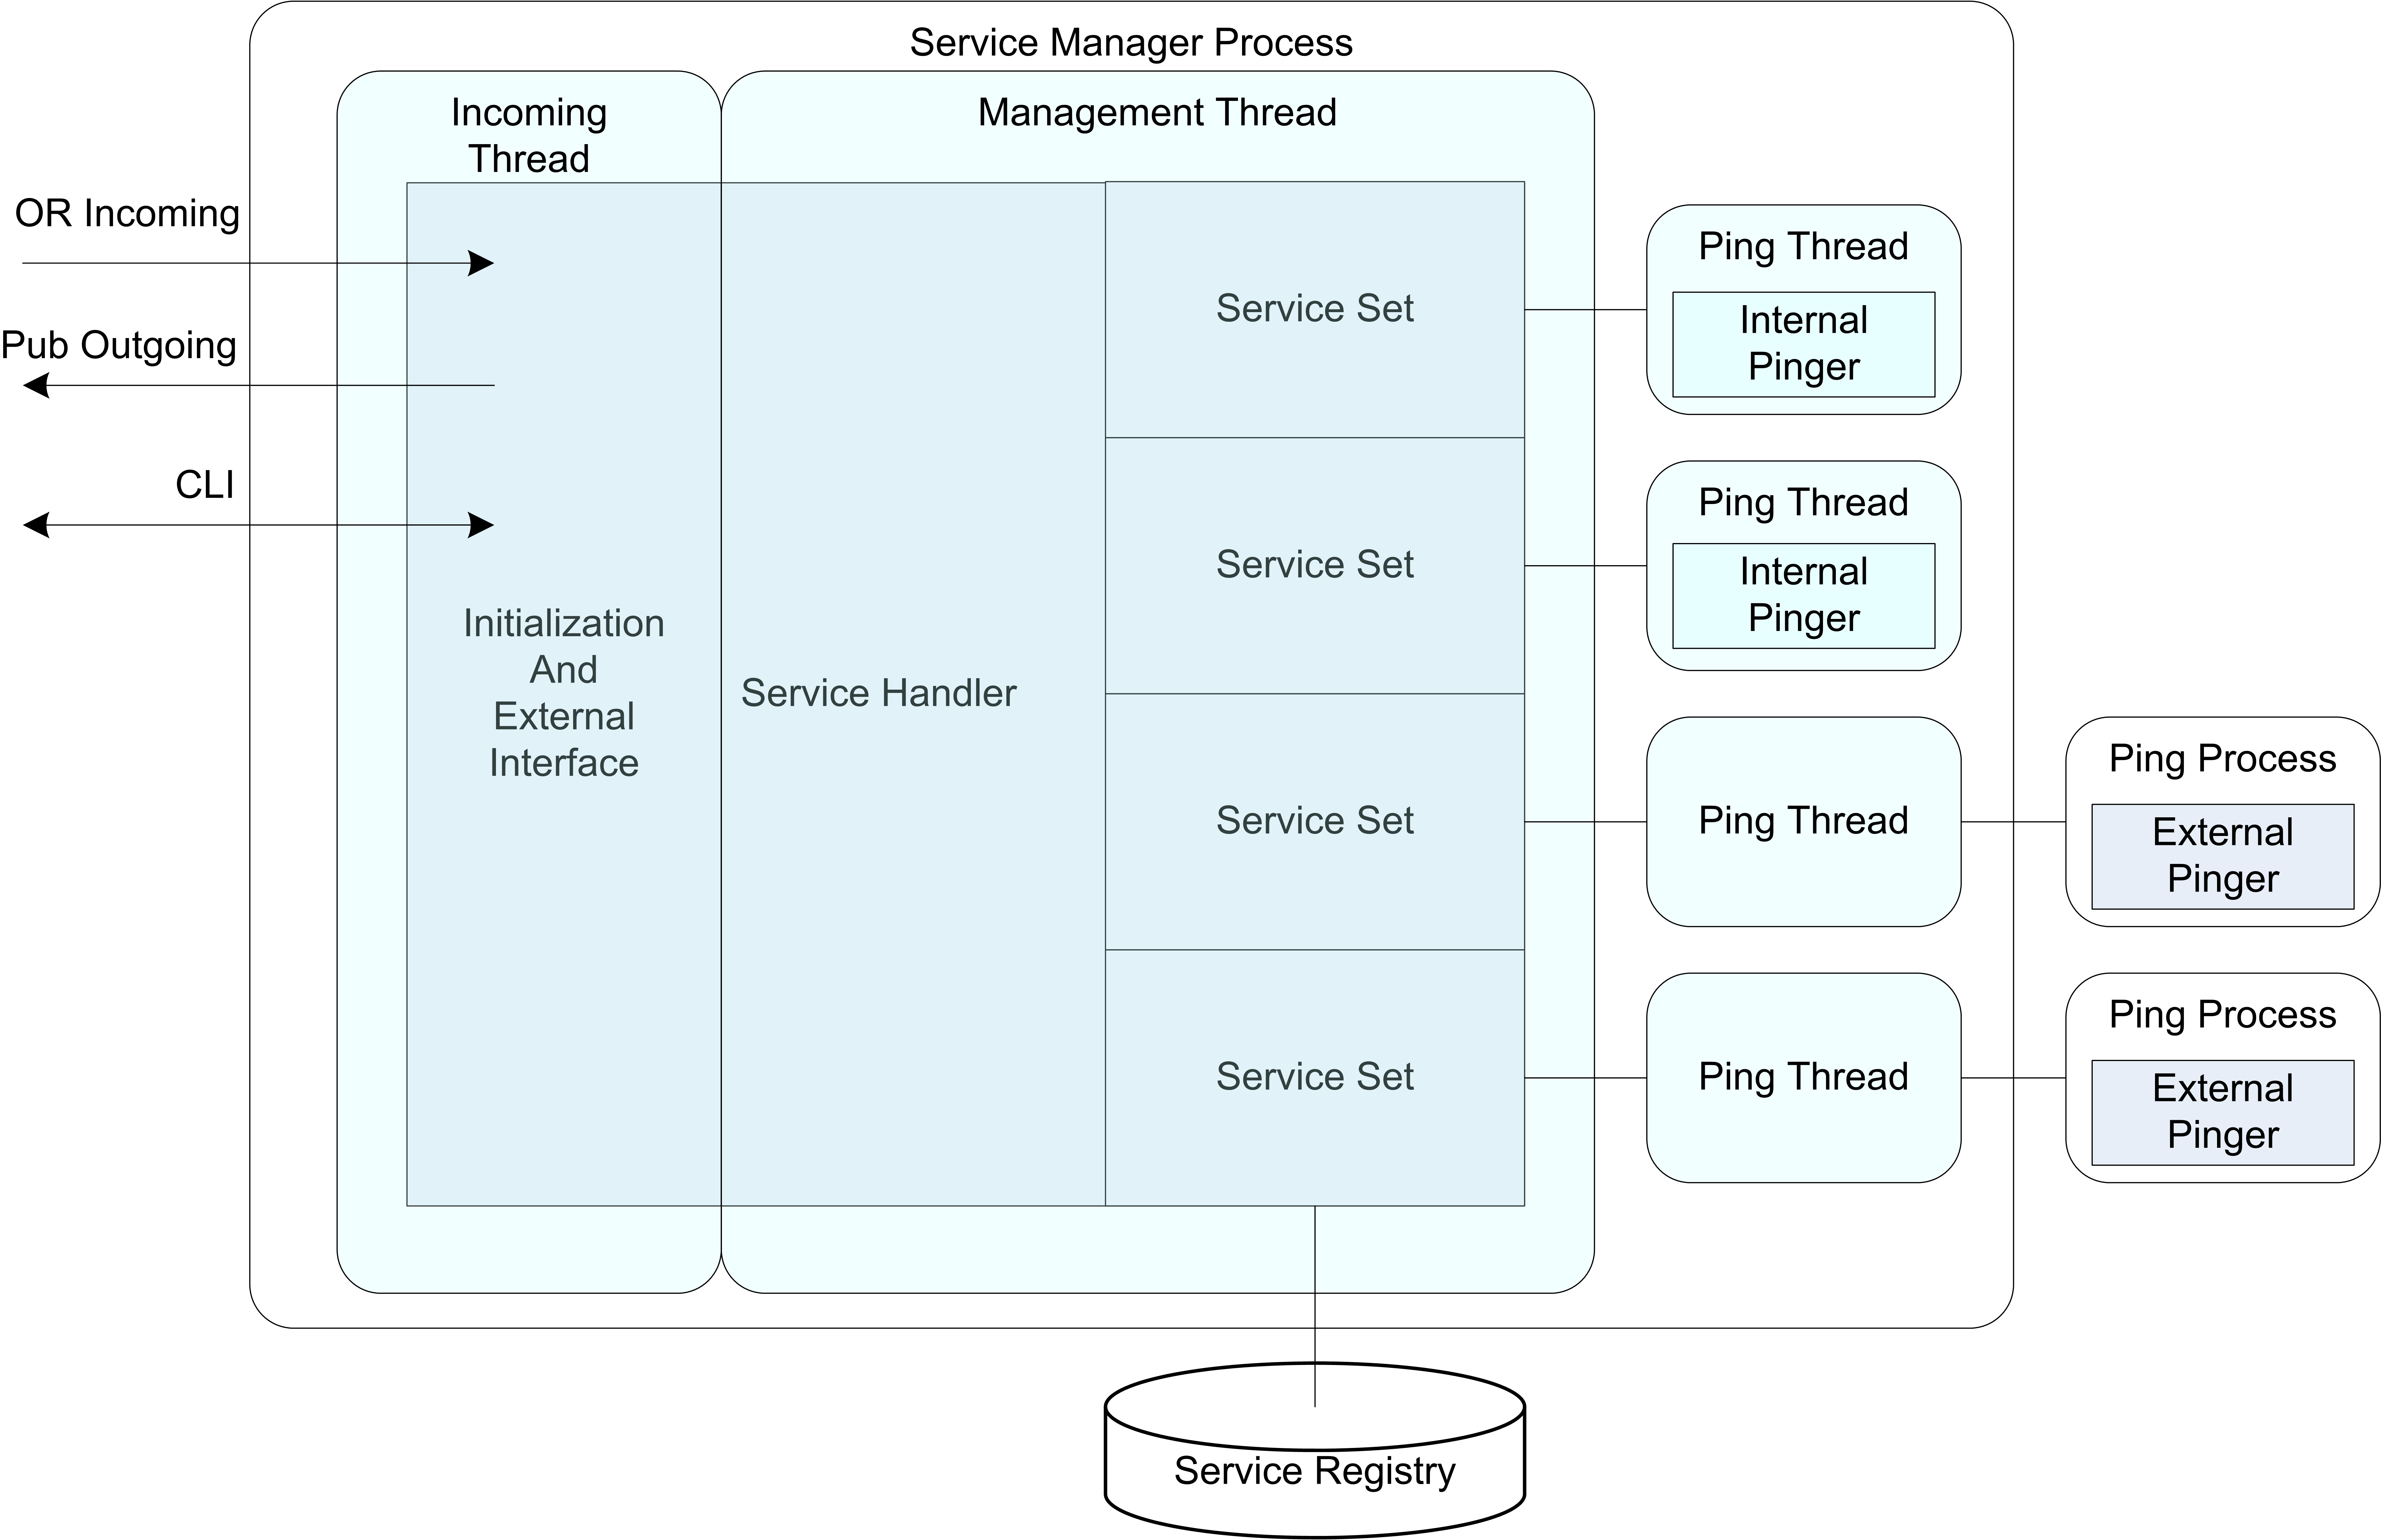
\includegraphics[width=5.5in]{images/ducc-internals/sm-structure.png}
      \caption{Service Manager Structure}
      \label{fig:sm-structure}
    \end{figure}

   The terminology around Services can be confusing.  We review the ideas here.

   There are three ``countable'' entities involved in services.  
   \begin{description}
     \item[Service Registration] When a service is ``registered'' the Service Manager assigns
       a new, unique {\em Registration ID} to the registration.  This ID is associated with, and
       remains with, the service throughout its lifetime and beyond when it is archived.

     \item[Service Instance] When the Service Manager starts a service it issues a series of
       ``submit'' orders to the Orchestrator, one for each {\em Service Instance}.  All these 
       instances are associated with the {\em Service Registration}.  The orchestrator assigns
       a unique ID to each service instance, which is also permanently associated with that entity.
       
       This is analogous to a {\em job}, but with a single allocation.  The SM organizes
       multiple {\em Service Instances} under a single {\em Service Registration}.
       
     \item[Share Id] When an instance is submitted to the Orchestrator, the Orchestrator
       ``submits'' a request to the Resource Manager to find resources.  Each instance is
       treated independently by the RM.  When a resource is found for the instance, the RM
       assigns a {\em Share ID} to the allocation. 
       
       This is analagous to a {\em job's} process or ``PE''.
    \end{description}

    The {\em Service Registration} ID appears on the Services' page of the webserver.  The {\em
      Service Instance} ID and the {\em Share Id} appear in the ID column of the service details in
    the DUCC webserver.  For example, this ID: {\tt 289661.34094} indicates {\em Service Instance}
    ID {\tt 289661} and {\em Share Id} {\tt 34094}.

\section{Initialization and Interaction with DUCC}
   The component responsible for initialization and external interaction is
   implemented in the source file {\em ServiceManagerComponent.java}.  This
   straightforward bit of code performs the following functions, details of which
   are easy to understand by reading the source code itself.  

   \begin{description}
     \item[Initialization] This consists of the methods init() and
       start(). The DUCC framework instantiates ServiceManagerCompoent and calls
       its start() method.  This initializes various structures from
       {\em ducc.properties}, initializes the database connection, and
       initializes the two main threads:
       \begin{enumerate}
         \item The SM proper, {\em ServiceManagerComponent}, which
           fires its {\em run()} method which in turn calls {\em init()}.
           \item The Service Instance manager, implemented in {\em ServiceHandler.java}.
       \end{enumerate}
       The {\em init} method reads all registrations from its state repository and
       passes them to {\em register()} (using the same code path as the {\em register} CLI),
       to establish them in a memory map and possibly initialize them.


       \item[Interaction With DUCC] There are three primary interactions to be aware of:
         \begin{enumerate}
           \item Incoming Orchestrator publications.  This arrives on an external
             communication thread  and passed to
             the method {\em orchestratorStateArrives} which, if it accepts the
             publication, saves the incoming publication and issues a {\em notify()} to 
             the main {\em ServiceManagerComponent} thread to allow processing of the state.  

             The method {\em processIncoming} is then called which does standard DUCC
             state-differencing and passes updates to the {\em Instance Management} code
             in {\em ServiceHandler}.

           \item CLI requests.  These are passed via the usual DUCC event handlers to specific
             second-level handlers, one for each type of CLI request (e.g. {\em register()}).  Each of these
             second-level handlers is responsible for these actions:
             \begin{description}
               \item[User validation.]  Insure the caller of the CLI is {\em authenticated}, i.e.
                 is the user he claims to be.
               \item[Ducc is running.]  The DUCC Orchestrator must be actively publishing state
                 before SM is allowed to interact with users.                 
             \end{description}
             
             If these simple tests are passed, the request is passed to the Instance Management
             code in {\em ServiceHandler} to check for authorization (i.e. is this user allowed
             to perform this action against this service).  

           \item Outgoing state publications.  Outgoing state is a simple map, one entry per
             job (a ``job'' for SM is any unit of work in the system: UIMA-AS job, Service instance,
             Reservation, AP).  The entry contains the state of the job relative to any
             services it depends on, which is interpreted by the Orchestrator and Web Server.

         \end{enumerate}

         Note that Orchestrator publications and CLI requests may be ignored under these two conditions:       
         \begin{enumerate}
         \item SM initialization is not complete.  Completion is flagged as the last
           action of {\em init()}.
         \item RM has not yet assigned the JD node.  The incoming OR publication includes a flag to
           indicate whether the JD node is assigned.  We have to wait here because we do not want
           the SM to process work or initialize any services until it is confirmed that the system
           is fully initialized.  Note that this minimizes the occurrence of errors and simplifies
           error management because you can all errors occurred in a fully initialized environment.
         \end{enumerate}
         
     \end{description}
   

\section{Service Instance Management: ServiceHandler and ServiceSet}
    After the differencing engine has determined the various work events that have
    occurred, the Service Instance Management code examines each event
    and acts upon it.  

\subsection{Operational Overview}
    The code described below runs in a thread separate from the main thread
    described in the previous section.  Incoming events are placed on lists
    segregated by function (a list for new Jobs, a list for updated Jobs, etc).  As soon
    as all incoming events are placed on these lists the {\em Service Instance Management}
    thread is {\em notified}.  The {\em Service Instance Management} thread sets a lock,
    drains the lists into internal structures, and releases the lock.  This segregates the
    the actions of the {\em ServiceManagerComponent} from {\em Service Instance Management}.

    As incoming events are acted upon, a summary of the service state for all
    incoming work is built up.  After all events are processed, the {\em ServiceManagerComponent} 
    (previous section) is notified and the state publication is sent to the Orchestrator.

    There are two primary components involved in {\em Service Instance Management:}
    \begin{description}
      \item[ServiceHandler.java] This is a singleton object which runs in its own 
        thread sepparate from the {\em ServiceManagerComponent}.  It fields the
        updates from the Orchestrator and CLI, resolves Service dependencies, and signals
        the {\em ServiceSet} for each affected service so appropriate action can be taken.
        It maintains all the records of registered services and service-dependent jobs
        in an inner class {\em ServiceStateHandler}.
      \item[ServiceSet.java] There is one {\em ServiceSet} for every registered service.  It is
        instantiated on receipt of a registration and destroyed only when a service is unregistered.
        It is responsible for submitting service instances to the Orchestrator, reacting to state
        changes of the Service Instances, enforcing management policies ({\em reference start}, {\em
          autostart}, {\em manual start}), and fielding the data from the service Pinger.
    \end{description}
      
\subsection{ServiceHandler.java}
    The work-related events, fielded by {\em ServiceHandler}, are described below.
    These events can be placed into two broad categories:
    \begin{enumerate}
      \item Events relating to work that requires services, usually UIMA-AS jobs
      \item Events relating to service instances for registered services.  
    \end{enumerate}
    
    Within each category are three types of interesting events.
    \begin{enumerate}
      \item A new job or service instance has entered the system.  This is essentially a REQUEST
        from the Orchestrator, asking if all necessary services are available.  No work
        has been started in the system, and will not be until SM responds ``services available''
        to the request.

        NOTE that the Orchestrator has a ``fast-path'' for work that has no service dependencies, in
        that it does not wait for the SM to respond regarding such work.  SM does in fact respond,
        but after the fact, and the response is not used.

      \item An existing job or service instance has changed state.  This is work that the 
        Orchestrator has started: there are physical processes either started, or in the act
        of starting and their states may be evolving.

      \item An existing job or service instance has terminated.
    \end{enumerate}
    
    While technically any type of DUCC work can be dependent on a service, by far the most common
    is UIMA-AS Jobs and Service instances.  The SM must treat work which IS a Service Instance
    a little differently from all other work (because all work is potentially depdenent on the
    state of Service Instances). Below we will use the term ``Job'' to refer to any
    kind of work that is not a service instance.

    NOTE: for simplicity, the descriptions in this section use the term ``services available'' to refer
    to the single state {\em Available} which indicates a service is running and is successfully
    pinging, and  ``services unavailable'' to refer to all other states.  The complete set of
    states is encoded in the class
\begin{verbatim}
org.apache.uima.ducc.transport.event.sm.IService.java
\end{verbatim}
    in the enum {\tt ServiceState} as shown below.
\begin{verbatim}
    public enum ServiceState 
    {
      Pending,        // Work is waiting on at least one service to start
      Waiting,        // A job is waiting on at least one service to ping
      Starting,       // Instance is started, but not yet to Initializing
      Initializing,   // A job is waiting on at least one service to initialize
      Available,      // All services for this job are active and pinging, or else
                      //     no services are needed for the job
      NotAvailable,   // SM to OR only: reference to a non-existent service 
      Stopped,        // The service is not started
      Stopping,       // Service is told to stop but it takes a while
      Undefined,      // Catch-all, means basically "who cares"
      ;
    }
\end{verbatim}

    \paragraph{Service Events}. Service events are {\em processed in the order shown
    below.} The order is important because overall service state is advancing through the
    first three events.
    
    \begin{description}
      \item[A new Service Instance has arrived.]  The associated {\em ServiceSet}
        is found and signalled.  If the associated {\em ServiceSet} cannot be found this
        is considered a ``rogue'' service instance and is ignored.  This occurs if
        the incoming process cannot be matched with a registered service; for example, if
        the {\em DuccServiceSubmit} CLI is called outside of SM.  Usually this is an
        error condition but is not considered fatal by SM.

        If this service is dependent on other services, the {\em ServiceSet}s for those
        other services are fetched and signalled, which may in turn cause additional
        service instances to be submitted.  If all of these other services are Running,
        the new service is marked ``services available'' and the Orchestrator will 
        physically start the new instance.  Otherwise it is marked ``services unavailable''
        and will not be allowed to start until it's own service dependencies are running.

        Note how this implements a sort of ``domino'' effect for starting services.  Suppose
        you have two services, A dependent on B, and a job dependent on A,
        with none of these running.  When job A arrives at SM it is marked ``services unavailable'' and
        service A is submitted.  When service A arrives from Orchestrator it is marked ``services unavailable'' and
        service B is submitted.  When service B arrives from Orchestrator it is marked ``services available'' so 
        that Orchestrator may start it.  When it starts, service A is marked ``services available'' and is
        started by Orchestrator.  When service A starts, the job is finally marked ``services available'' and
        is allowed to start.

        As mentioned above, if the services is NOT dependent on other services, the Orchestrator
        will fast-path its start, and SM will mark it ``services available''.
     
      \item[An existing Service Instance has arrived.]  The {\em ServiceSet} is
        fetched and signalled with the state of the incoming instance.  This may cause
        the Service State to be updated, for example from Initializing to Running.  Pingers
        may be started as needed.

        Note that, because this is processed BEFORE jobs are processed, job state may be
        updated from ``services available'' to ``services unavailable'' (or vice-versa).

      \item[A Service Instance has exited.]  Some service instance for some managed
        service has exited for some reason.

        The associated {\em ServiceSet} is found and signalled.  The {\em ServiceSet}
        takes appropriate action, restarting the instance if the exit
        was unexpected, or perhaps simply updating its records if the service is
        being stopped or the number of instances reduced.

      \item[A new job has arrived.]  
        The declared service dependencies are parsed and the {\em ServiceSet}
        object for each such service is signalled.   The {\em ServiceSet} increments the reference count for
        the service and, in the case of {\em reference-started}
        services, starts some number of instances (using the ``hidden'' CLI utility
        {\em DuccServiceSubmit}.

        Based in the current state of the service, the job is flagged with ``services available'' or
        ``services unavailable''.  The job is marked ``services available'' if-and-only-if all
        its declared services are started, in running state, and being successfully {\em tested} (``pinged'').

      \item[An existing job has arrived.]  Work that is not new may need its service state reevaluated.
        The declared service dependencies are parsed and the associated {\em ServiceSet}
        objects are fetched.  An analysis of the combined work states and service
        states is done.  The job is flagged ``services available'' or ``services unavailable''.

        Note that a job's service-state can change from ``services available'' to ``services
        unavailable'' if a service fails for some reason.

      \item[A job has exited.]  A job which might be dependent
        on a service has left the system. 

        The ServiceHandler examines all the declared services for the work.  For each
        dependency, if the service is started, the ServiceSet for the service is 
        signalled.  Each affected {\em ServiceSet} decrements its reference count.  If the
        count goes to zero, and if this is
        a reference-started service, the {\em ServiceSet} stops all instances.
          
    \end{description}
    
\subsection{ServiceSet.java}
{\em ServiceSet} is responsible for the care-and-feeding of the set of objects, threads, and
processes used to manage an individual service.  There is one {\em ServiceSet} instantiated for
every registered service.  {\em ServiceSet} does NOT run in its own thread.  Its methods are always
executed either on the thread of the {\em ServiceHandler} or on a {\em pinger} thread. It is
responsible for maintaining the correct number of running instances, fielding pings, and updating
the state repository (as of DUCC 2.1.0, a database) for a single service.

   The primary functions include:
   \begin{description}
     \item[Enforce Autostart]  If the service is registered for autostart, insure sufficient instances are started
       and start new ones if needed.  This is called at the end of each update cycle from the {\em ServiceHandler}.

     \item[Manage references] Maintain a reference count to reflect all work that is
       referencing the service.  If the service is ``reference started'' this can trigger
       the start of new instances and the shutdown of existing instances.  This count is
       always maintained so if the administrator changes the start-up policy for the service,
       the reference count is already correct and is used.

    \item[Start-up and hot start] On hot-start, the method {\em bootInstances()} is called to
      synchronize each service set with the incoming orchestrator publications, followed by
      bootComplete() to finalize bookkeeping and update the meta state data.

    \item[Field pings] When the Orchestrator state indicates that at least one instance for the
      service is in Running state, the {\em ServiceSet} starts a pinger.  After every ping,
      the pingers call {\em signalReblance()} to respond to the ping and enforce any
      potential state changes as a result of the ping, including starting and stopping 
      specific instances.

    \item[Sequence Instance Startup] The {\em ServiceSet} also sequences instance start-up so that
      in general, there is only a single instance starting at  time.  This is managed in the
      method {\em needNextStart()};

      Instances are sequenced up for several reasons:
      \begin{itemize}
        \item Avoid flooding the system with start requests during boot.
        \item Avoid start/fail loops with faulty services.
      \end{itemize}
      
    \item[Respond to Instance State Change]  The {\em ServiceHandler} invokes the {\em ServiceSet}
      method {\em signalUpdate} on every Orchestrator update.  This method examines the entire
      state of the service and coordinates any actions which may be triggered by state change
      of a service instance.

    \item[State Accumulation]  The state of a service is dependent on the cumulative states of
      all of its instances PLUS the state if its pinger.  The method {\em cumulativeJobState()}
      is responsible for state accumulation.

      The design point is that states are associated with an ordinal.  The larger the ordinal,
      the ``closer to functional'' a service is.  The lower the ordinal, the ``farther from functional''
      the service is.  State accumulation walks the states of all relevant components maintaining
      the {\em maximum} state encountered.  This {\em maximum} is considered to be the state of the
      service overall.  The method {\em translateJobState()} is used to assign the ordinal
      based on the state of the service instances.

    \item[State Management] There is a very simple state machine managed by two methods,
      {\em signal()} and {\em setState()}.  The details can be found by examining these methods.
      The design point is this:  most actions in the SM are considered {\em idempotent}.  Thus,
      regardless of the outcome of state change (or lack of state change), these actions are
      ALWAYS called; for example, ``start the pinger''.  The methods implementing the actions
      are responsible to determine whether the current situation is compatible with the requested
      action.  For example, if the method {\em startPingThread()} is called, that method must
      check to see if the ping thread is already running, and not start a new thread if so.

      This design makes the state machine extremely simple and easy to maintain.

      \item[Lingering Stop] {\em Lingering stop} occurs in a reference-started service when the
        final reference has exited.  It is implemented by a Java TimerTask, {\em LingerTask}.
        If the timer ``pops'', this task stops the service.  If a new reference arrives
        before the timer ``pops'', the task is canceled.

   \end{description}

\subsection{ServiceInstance.java}
    The {\em ServiceInstance} object is a simple helper whose responsibility it is to start
    a new instance.  It spawns a {\em DuccServiceSubmit} process as the user via {\em ducc\_ling} with a pointer to the
    registration properties, and scrapes the output in the response to get the Orchestrator-assigned
    ID.  The ID and any error messages are returned to the calling {\em ServiceSet}.

    This mechanism is used to manage ping-only services as well.  When a ping-only service is started,
    a subclass of ServiceInstance is started.  This {\em PingOnlyServiceInstance} simulates the start
    of an actual instance.  It maintains an internal thread that invokes {\em ServiceSet.signal()} to simulate
    the {\em ServiceHandler}'s regular state updates.  It is essentially a ``service proxy'' for the 
    non-DUCC-handled service that is being pinged, eliminating the need for most special cases in the
    handling of ping-only services.

\section{Service Health Management: Ping support}
    When the {\em ServiceSet} detects that at least one instance has achieved {\em Running} state,
    it calls the method {\em startPingThread()}.

    {\em startPingThread()} starts a thread dedicated to managing the pinger, with the class
    {\em PingDriver} running as its (logical) ``main''.  The {\em PingDriver} reaches back into its
    {\em ServiceSet} for the parameters needed to manage the pinger (Java class, ping interval,
    etc).

    The {\em PingDriver} implements two cases:
    \begin{enumerate}
      \item Internal pingers
      \item External pingers
    \end{enumerate}
    
    In both cases, the {\em PingDriver} object creates an object from {\em Ping.java}, loads
    the object with a {\em Map} of user and DUCC-supplied parameters, and passes the {\em Ping} to
    the ping implementation.  A timer is set and a response is waited for.  

    In both cases the ping mechanism collects ping parameters and passes them to the {\em AServicePing}
    object which was extended to create the pinger.  The ping mechanism then calls various
    methods on {\em AServicePing} to extract its state, constructs a {\em Pong} object, and uses
    this to communicate with the SM by invoking {\em ServiceSet.signalRebalance()}.  The details
    of how this occurs is different for internal and external pingers in the {\em PingDriver}.
    
    \subsection{Internal Pingers}

    If the pinger is registered as an ``Internal'' pinger, a Java ClassLoader is invoked to load
    the pinger's registered class. A timer loop is established to invoke the pinger.  On
    each invocation, the {\em PingDriver} directly invokes the methods on {\em AServicePing} 
    required to invoke the pinger and retrieve its state.  A {\em Pong} object is created
    from the state and passed to common code in the method {\em handleResponse()}.

    \subsection{External Pingers}

    If the pinger is registered as an ``External'' pinger, a ServerSocket is started and its listen
    port acquired. An instance of the class {\em ServicePingMain} is spawned under the identity of
    the owning userid of the service via {\em ducc\_ling}, passing the listen port and appropriate
    arguments needed to start the user's pinger. The stdout and stderr of the resultant process is
    captured and written to the SM log and the ping loop (describe below) is started.
    
    The {\em ServicePingMain} object receives a set of start-up parameters including the
    name of the user's ping class, classpath, start-up parameters, and endpoint.  The user's
    pinger, extending {\em AServicePing} is instantiated by {\em ServicePingMain} using a
    ClassLoader.  {\em ServicePingMain} then goes into
    an infinite, untimed loop waiting for the {\em Ping} requests from the {\em PingDriver}.  When
    a request arrives, the parameters in the request are gathered and sent to the user's pinger
    by calling methods on {\em AServicePing} as is done for internal pingers.
    The response is received and returned to {\em ServiceSet} in a {\em Pong} object.
    
    The embedded class {\em PingDriver.PingThread} is used to implement the protocol between SM and
    the external pinger.   The wire protocol between SM and {\em ServicePingMain} is quite simple.

    On the SM side:
    \begin{itemize}
      \item SM starts a ServerSocket and then issues an {\em accept()} waiting for the external pinger to connect.
      \item Once the pinger connects, enter a loop until terminated by SM:
        \begin{itemize}
          \item Write a new {\em Ping} object to the socket stream.
          \item Read a new {\em Pong} object from the socket stream.
        \end{itemize}
    \end{itemize}
    
    If SM terminates the pinger, the {\em Ping} object includes a flag that is read by
    {\em ServicePingMain} causing it to shutdown the user's pinger and exit.

    On the external pinger's side, with {\em ServicePingMain} started by {\em ducc\_ling} as
    the owner of the service:
    \begin{itemize}
      \item Read the command-line parameters and then:
        \begin{itemize}
          \item Connect to the SM on it's listen socket.
          \item Instantiate the user's ping class using a classloader.
        \end{itemize}
      \item Enter a loop:
        \begin{itemize}
          \item Read the next Ping
          \item If the Ping has the {\em exit} flag set, call the pinger's {\em stop()} method, close the
            input and output streams, and exit.
          \item Otherwise invoke the pinger's base methods defined in {\em AServicePing}.
          \item Construct a {\em Pong} object and write it to the SM's socket.
        \end{itemize}
      \end{itemize}
    

    \section{CLI Management}
    The CLI management code is relatively simple but has a few details worth mentioning.

    {\em ServiceManagerComponent} receives the incoming CLI call, insures the user identified
    in the incoming packet is the one who submitted it, that the DUCC Orchestrator processes
    is functioning, and passes the incoming packet to {\em ServiceHandler}.  Each different
    CLI function is passed to the appropriate second-level handler in {\em ServiceHandler}; for
    example, a registration request is passed to {\em ServiceHandler.register()}.

    Secondary vetting of the incoming request is then performed: 
    \begin{itemize}
      \item Check to see if the service exists.  If so, and it's a registration then fail with a
        ``duplicate services'' message.  If it is NOT a registration and it does not exist, fail with a
        ``service not found'' message.
      \item Insure the caller is authorized for the desired action (e.g. is the caller an
        admin or owner for the service).
      \item If the request can be performed immediately, do so and return confirmation.  These requests are
        \begin{itemize}
          \item Register
          \item Query
          \item Enable
          \item Disable
          \item Ignore references
          \item Observe references
        \end{itemize}
      \item If the request can take an arbitrarily long time, then build a deferred CLI object
        and enqueue it.  This deferred object is implemented in {\em ApiHandler.java}.  Return
        confirmation to the user that the request is accepted.  These requests are
        \begin{itemize}
          \item Start
          \item Stop
          \item Modify
          \item Unregister
        \end{itemize}
        
    \end{itemize}
      
    Deferred requests are dequeued and executed one at a time.  The user is not directly
    informed of this execution as it may complete at an arbitrary time in the future.  For
    example, stopping or unregistering a service both involve an elaborate sequence of
    actions to stop the processes, deallocate the space, and update the SM records.
    Starting a service is also quite elaborate and additionally, service starts are
    sequenced so they are submitted one-at-a-time; services with many instances can take
    a significant time to fully start.

    These requests are synchronized with other SM activities to minimize race conditions by
    handling them in the same execution thread in {\em ServiceHandler} that is handling incoming Orchestrator
    publications.  Deferred requests are implemented in two methods each:
    \begin{enumerate}
      \item An ``immediate'' method which vets the CLI parameters, constructs, and enqueues the deferred request:
        \begin{itemize}
          \item ServiceHandler.start()
          \item ServiceHandler.stop()  
          \item ServiceHandler.modify()
          \item ServiceHandler.unregister() 
          \end{itemize}                      
      \item A ``deferred'' method, invoked from the deferred request:
        \begin{itemize}
          \item ServiceHandler.doStart();
          \item ServiceHandler.doStop();
          \item ServiceHandler.doModify();
          \item ServiceHandler.doUnregister();
        \end{itemize}
        
    \end{enumerate}
    
